\documentclass{beamer}
% Prévoir à peu près un transparent par minute d'exposé.
% Deux ou trois sections semble être une bonne chose.
\mode<presentation>
{
	\usetheme{Warsaw}
	\setbeamercovered{highly dynamic}
	\setbeamercovered{invisible}
}

\usepackage[english]{babel}
\usepackage[utf8]{inputenc}
\usepackage{multimedia}

%\usepackage{hyperref}

\setbeamersize{text margin left=20pt}
\setbeamersize{text margin right=20pt}

\defbeamertemplate*{footline}{infolines theme}
{
	\leavevmode%
	\hbox{%
		\begin{beamercolorbox}[wd=.33\paperwidth,ht=2.25ex,dp=1ex,center]{author in head/foot}%
			\usebeamerfont{author in head/foot}G. Lesauvage
		\end{beamercolorbox}%
		\begin{beamercolorbox}[wd=.33\paperwidth,ht=2.25ex,dp=1ex,center]{title in head/foot}%
			\usebeamerfont{title in head/foot}\insertshorttitle
		\end{beamercolorbox}%
		\begin{beamercolorbox}[wd=.33\paperwidth,ht=2.25ex,dp=1ex,right]{date in head/foot}%
			\usebeamerfont{date in head/foot}September 12$^{th}$-14$^{th}$, 2011\hspace*{2em}
			\insertframenumber{}/\inserttotalframenumber\hspace*{2ex}
		\end{beamercolorbox}
	}%
	\vskip0pt%
}

\date{\tiny September 12$^{th}$-14$^{th}$, 2011}
\title[HMS 2011]
{
	$D^2CTS$ : a Dynamic and Distributed Container Terminal Simulator
}

\author
{
	S. Balev, F. Guinand and G. Lesauvage
}

\institute[LITIS]
{
	
 \begin{columns}
 		\begin{column}[l]{6cm}
 			\begin{center}
 			
\includegraphics[height=.1\textheight]{fig/logouniversiteduhavre.png} \\
 			\tiny\textit{Unit\'{e} de Formation et de Recherche des Sciences et Techniques}
 			\end{center}
 		\end{column}
 		\begin{column}[r]{6cm}
 			\begin{center}
 			
\includegraphics[height=.135\textheight]{fig/logolitis.png} \\
 			\tiny\textit{Laboratoire d'Informatique et du Traitement de l'Information et des Syst\`{e}mes}
 			\end{center}
 		\end{column}
 \end{columns}

 	
}

\normalsize

  \AtBeginSection[Plan]
  {
  \begin{frame}<beamer>
  \frametitle{Plan}
  \tableofcontents[currentsection]
  \end{frame}
  }
\setbeamertemplate{blocks}[rounded][shadow=true]
\subject{HMS 2011 ROME}
\begin{document}

\begin{frame}
\titlepage
\end{frame}

\begin{frame}
\frametitle{Plan}
\tableofcontents
\end{frame}

\section{Introduction and Objectives}
\begin{frame}{The CALAS project}
\begin{columns}
    \begin{column}[l]{5.5cm}	
	\begin{itemize}
		\item CArrier LAser tracking

		\item Companies : 
			\begin{itemize}
			 \item LDTT
	 		 \item EADS/Astrium
			\end{itemize}

		\item Laboratories : 
			\begin{itemize}
			    \item LMAH
			    \item LITIS
			\end{itemize}
	\end{itemize}
    \end{column}
    \begin{column}[r]{4.5cm}
		\begin{flushright}
		  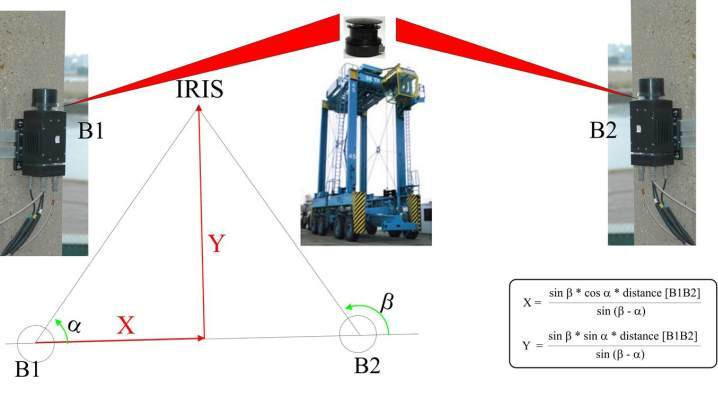
\includegraphics[height=.30\textheight]{fig/angles.jpg}
		\end{flushright}
    \end{column}
 \end{columns}	
  \pause
  \begin{block}{CALAS Objective: }
		\begin{center}
			To know the state of the terminal, in real time, for both containers and handling trucks location\\
		\end{center}
  \end{block}


\end{frame}

\begin{frame}{$D^2CTS$}

  \begin{center}
Dynamic and Distributed Container Terminal Simulator\\
  \end{center}
  \begin{block}{Objectives: }
   	\begin{minipage}[]{\columnwidth}
	  \begin{itemize}
		\item Emulating a container terminal in both its structure and its dynamics\\
		\pause
		\item Performing various optimization algorithms in a realistic environment for testing their relevance\\
	  \end{itemize}
\end{minipage}
  \end{block}
\end{frame}


\section{Modelling}
  \subsection*{Structure}
 \begin{frame}{Test Case : Terminal de Normandie (Le Havre, France)}
   \begin{center}
	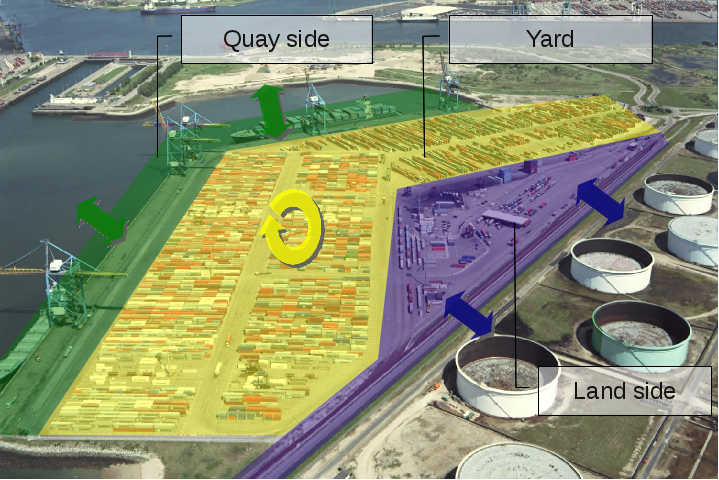
\includegraphics[height=.60\textheight]{fig/3zonesOfTN.png}
  \end{center}   
 \end{frame}


  \begin{frame}{Road network}
\begin{columns}
    \begin{column}[l]{4.0cm}	
	\begin{itemize}
	  \item Crossroads
	  \item Roads
	  \item Road points
	  \item Lanes
	\end{itemize}
    \end{column}
    \begin{column}[r]{6.5cm}
	\begin{flushright}
	  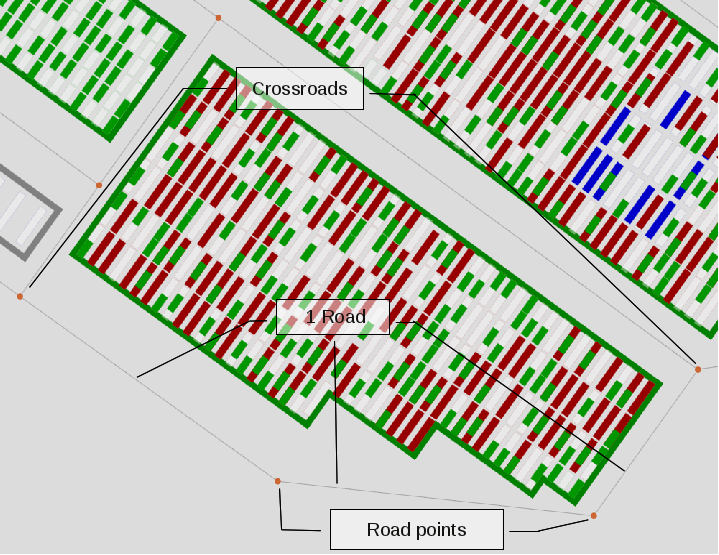
\includegraphics[height=.55\textheight]{fig/FigRoadPoints.png}
	\end{flushright}
    \end{column}
 \end{columns}	
    
 \end{frame}

\subsection*{Laser Localizing System}
\begin{frame}{Laser localizing system}
  \begin{columns}
   
    \begin{column}[l]{6cm}
	  \begin{center}
	  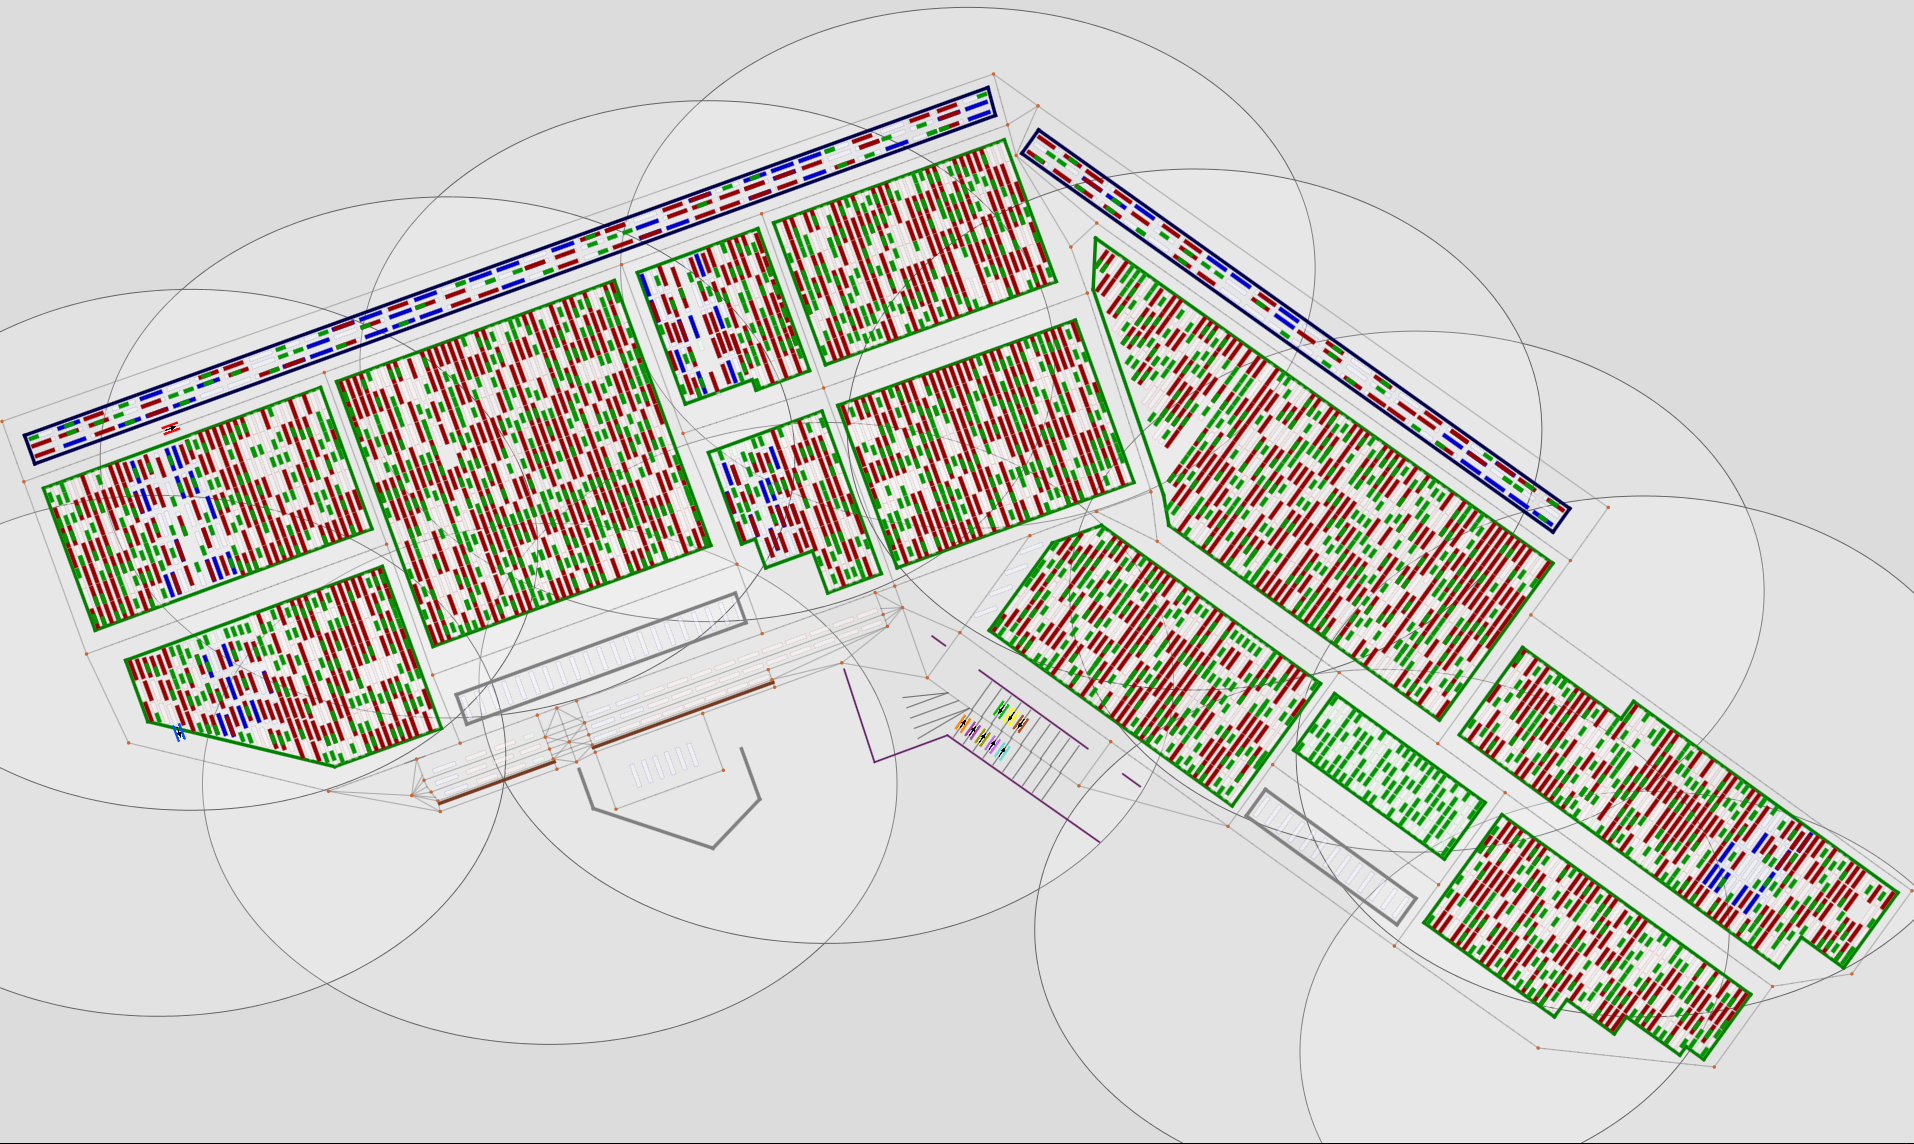
\includegraphics[height=.50\textheight]{fig/captureBornesLaser.png}
	  \end{center}
    \end{column}
    \begin{column}[r]{4.5cm}	
      \begin{flushright}
	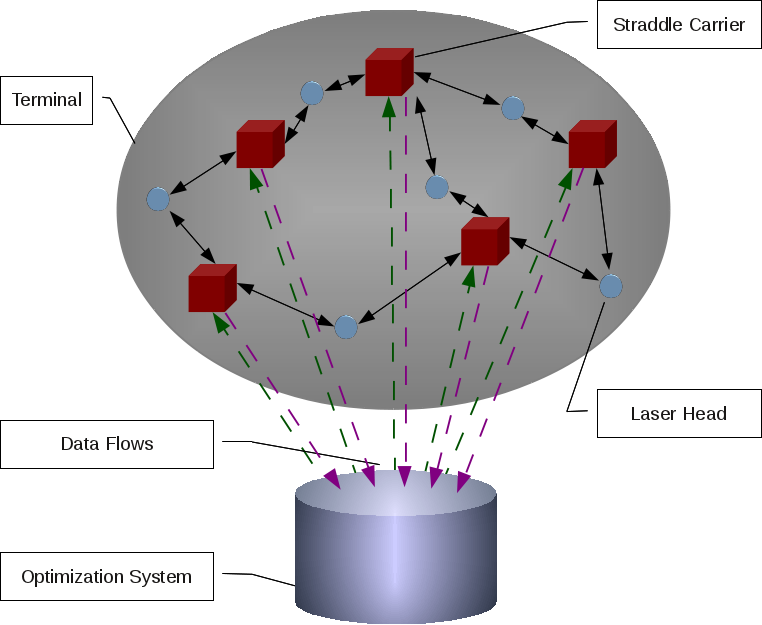
\includegraphics[height=.50\textheight]{fig/communicationsEN.png}
      \end{flushright}
    \end{column}
 \end{columns}	
  \begin{columns}
   
    \begin{column}[l]{7cm}
	  \begin{center}
	   \tiny \textit{Laser localizing system modelling on the Terminal de Normandie}
	  \end{center}
    \end{column}
    \begin{column}[r]{4.5cm}	
      \begin{flushright}
	\begin{center}
	   \tiny \textit{Communications between the straddle carriers and the optimization system}
	  \end{center}
      \end{flushright}
    \end{column}
 \end{columns}	

\end{frame}

 \subsection*{Mobility}
  \begin{frame}{Mobility}
  
  \begin{center}
  Only straddle carriers mobility is handled by the simulator for the moment
\vspace{0.8cm}

\begin{columns}
    \begin{column}[l]{3.0cm}	
      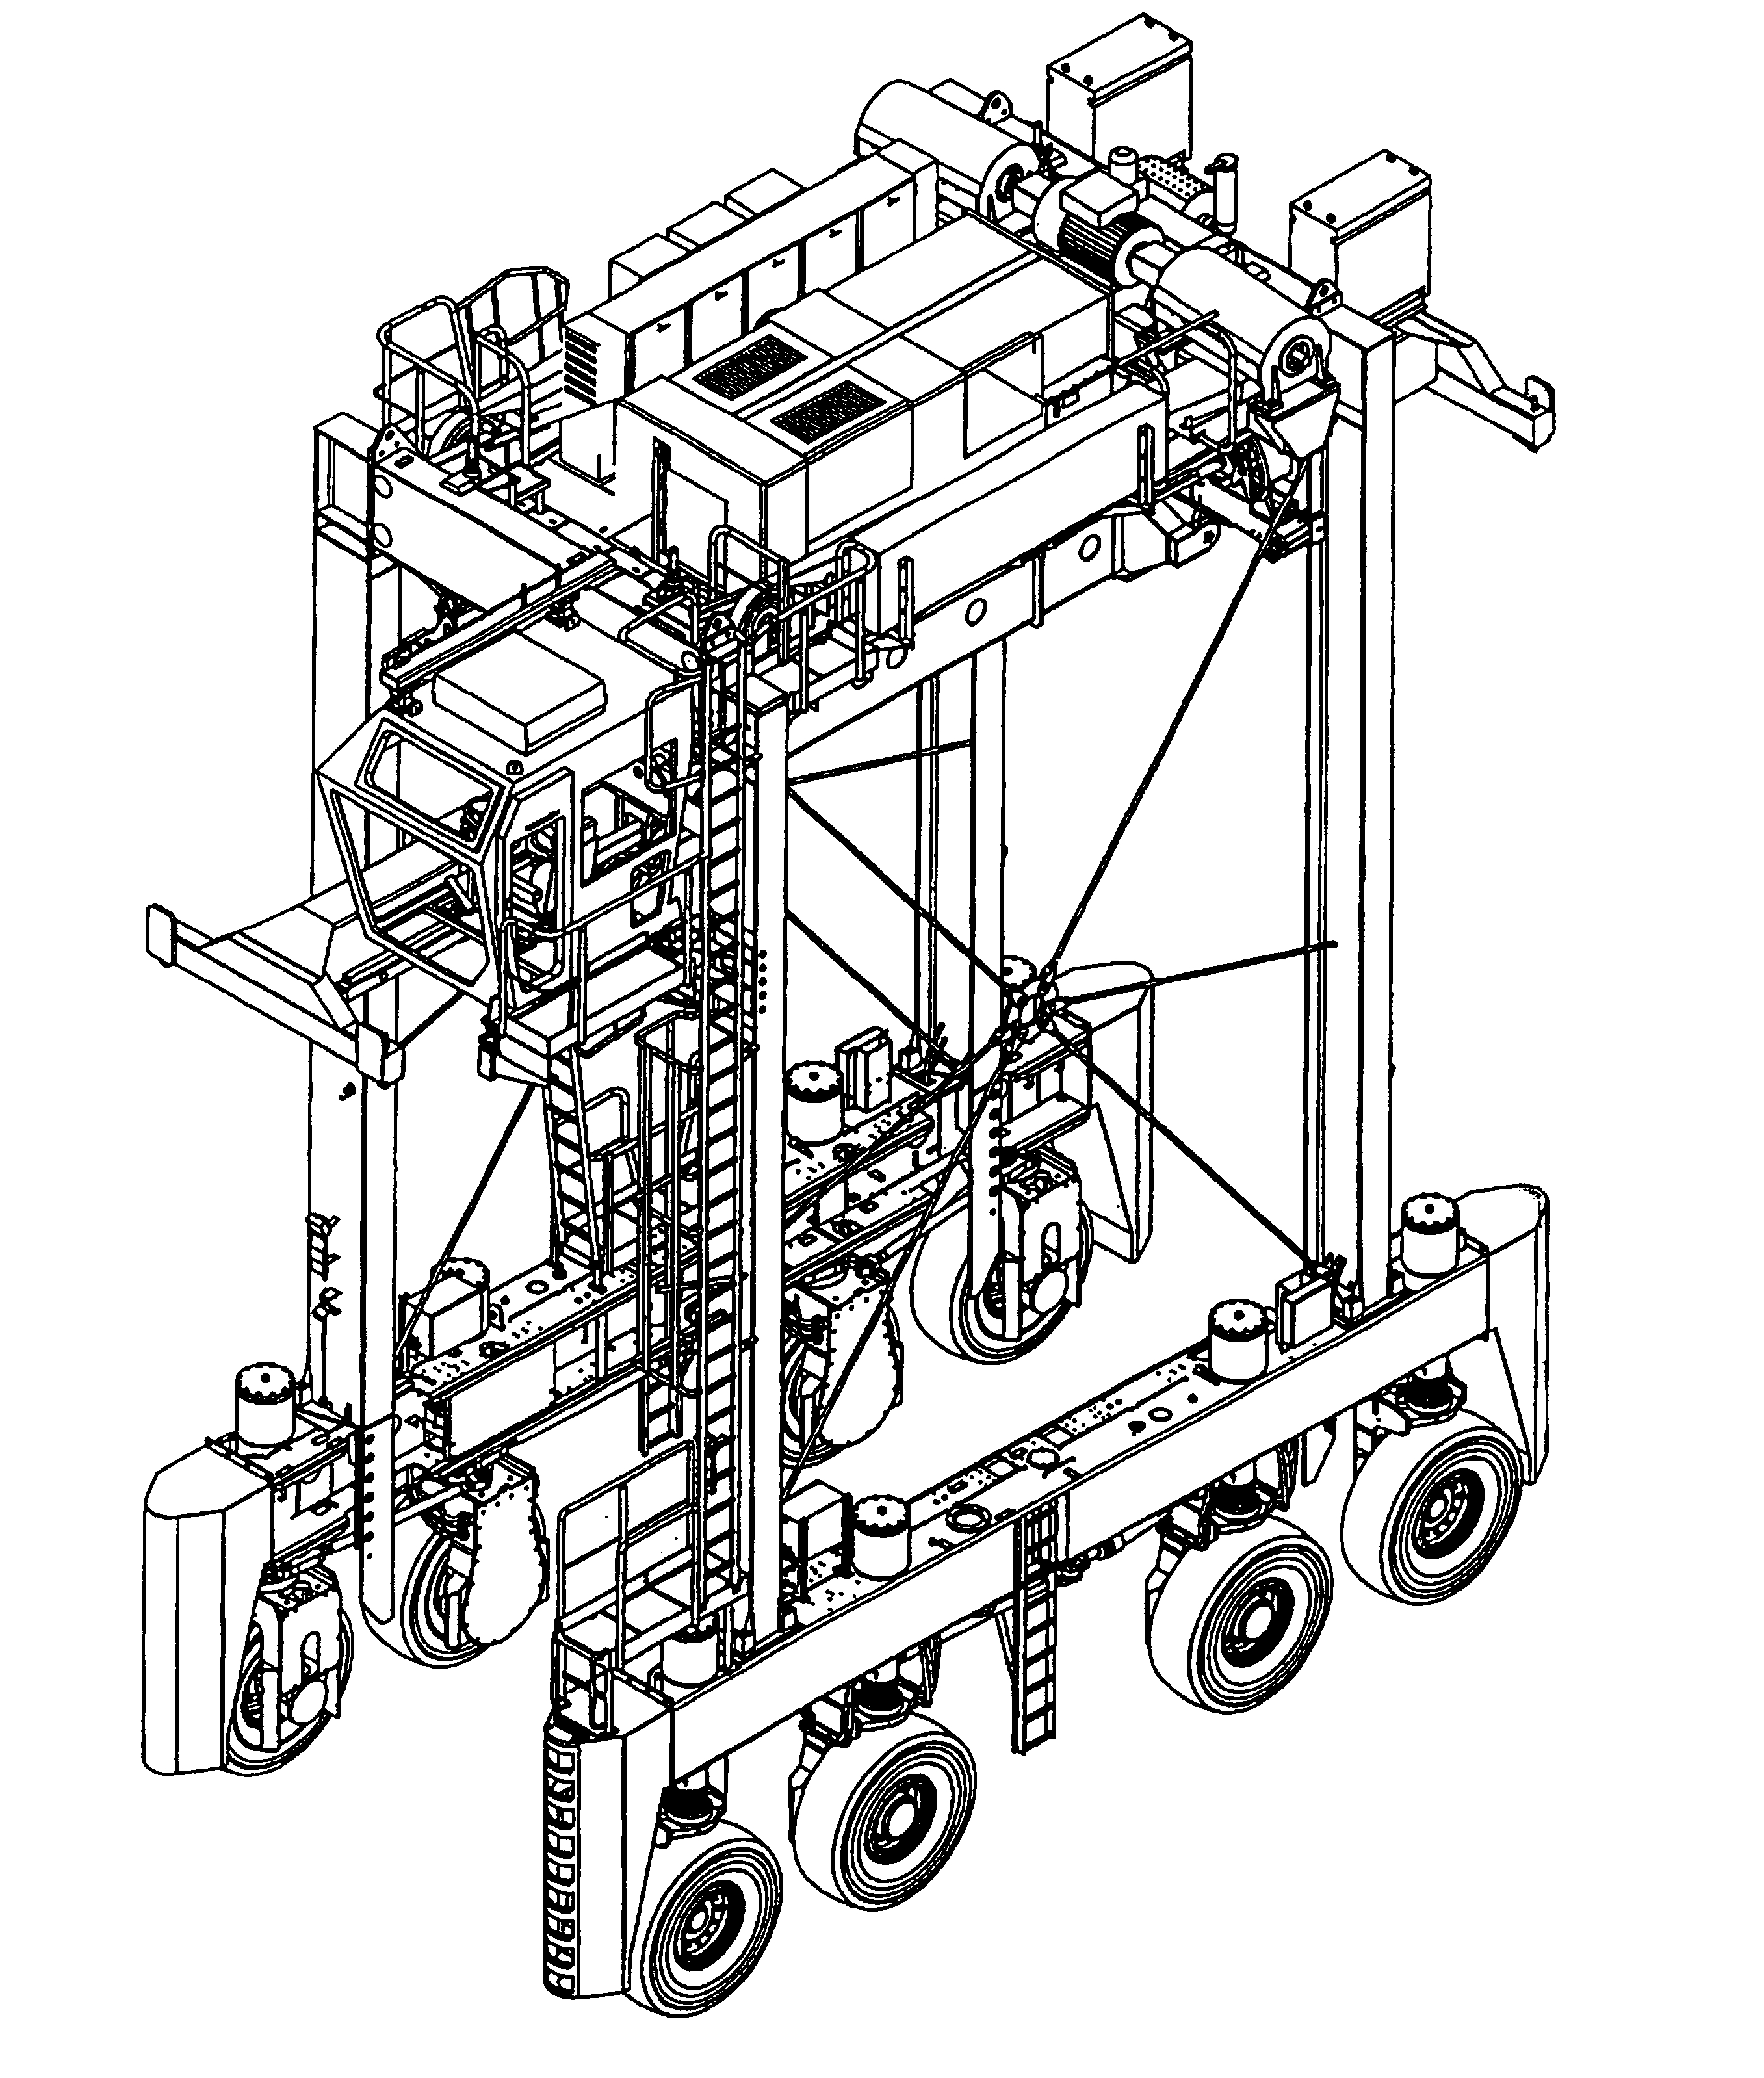
\includegraphics[height=.25\textheight]{fig/schema_sc.jpg}
    \end{column}
    \begin{column}[c]{4.0cm}	
      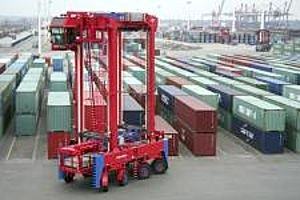
\includegraphics[height=.25\textheight]{fig/chariot_cavalier.jpg}
    \end{column}
    \begin{column}[r]{3.0cm}	
      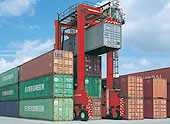
\includegraphics[height=.25\textheight]{fig/tn-straddle-carriers.jpg}
   \end{column}
\end{columns}
  \end{center}
\begin{itemize}
   \pause \item on roads: straddle carriers can pass and overtake each other
   \pause \item on lanes: straddle carriers can neither pass nor overtake each other
 \end{itemize}
\begin{center}
\pause $\Rightarrow$ Lanes are modelled by FIFO arcs
 \end{center}
 \end{frame}
\begin{frame}{Straddle Carrier's activity}
  \begin{itemize}   
   \item For a straddle carrier, a mission consists in moving a container
   \pause
    \item 3 kinds of missions : 
    \begin{itemize}
      \item Loading a ship, a train or a truck
      \pause
      \item Unloading a ship, a train or a truck
      \pause
      \item Optimizing the yard
    \end{itemize}
\end{itemize}
\end{frame}

  \subsection*{Time modelling}
\begin{frame}{Time modelling}  
  \begin{itemize}
   \item Discrete time
   \item The step size is set before starting simulation
  \end{itemize}
\end{frame}

\begin{frame}{Video : time control in D$^2$CTS}
   \begin{center}
       \movie[height=0.8\textheight,showcontrols,poster,autoplay]{
\includegraphics[height=0.8\textheight]{fig/videos/posterTimeControl.jpg}}{fig/videos/timeControl.mpg}
   \end{center}
\end{frame}

  \subsection*{Events}
  \begin{frame}{The events}
   \begin{itemize}
    \item Mission event: arrival, cancellation, delay
    \pause
    \item Vehicle arrival/departure
    \pause
    \item Straddle carrier failure:
	  \begin{itemize}
	      \item  Physical failure (motor, spreader or both) \hyperlink{Straddle Carrier Failure}{\beamerbutton{video}}	%TODO : Video of a straddle carrier failure
	      \item The driver does not choose the mission proposed by the scheduler
	      \item The driver does not follow the computed route
	  \end{itemize}
    \end{itemize}
  \end{frame}

\begin{frame}{Video : Straddle Carrier Failure}
  \label{Straddle Carrier Failure} 
  \begin{center}
       \movie[height=0.8\textheight,showcontrols,poster,autoplay]{
\includegraphics[height=0.8\textheight]{fig/videos/posterTimeControl.jpg}}{fig/videos/SCFailure.mpg}
   \end{center}
  
  \begin{center}
    \hyperlink{callSCF}{\beamerreturnbutton{}}
  \end{center}

\end{frame}

  \begin{frame}
    \label{callSCF}
   \begin{itemize}
    \item Mission event: arrival, cancellation, delay
    \item Vehicle arrival/departure
     \item Straddle carrier failure:
	  \begin{itemize}
	      \item  Physical failure (motor, spreader or both) \hyperlink{Straddle Carrier Failure}{\beamerbutton{video}}	%TODO : Video of a straddle carrier failure
	      \item The driver does not choose the mission proposed by the scheduler
	      \item The driver does not follow the computed route
	  \end{itemize}
    
    \pause
    \item Container loss within the terminal	%TODO !!!
    \pause
    \item Laser head failure (range reduction from 100\% to 0\% ) \hyperlink{Laser Head Failure}{\beamerbutton{video}}%TODO : Video of laser head failure
   \end{itemize}
  \end{frame}
  
\begin{frame}{Video : Laser Head Failure}
  \label{Laser Head Failure} 
  
  \begin{center}
       \movie[height=0.8\textheight,showcontrols,poster,autoplay]{
\includegraphics[height=0.8\textheight]{fig/videos/posterTimeControl.jpg}}{fig/videos/LHFailure.mpg}
   \end{center}
  
  \begin{center}
    \hyperlink{callLHF}{\beamerreturnbutton{}}
  \end{center}
  
  \end{frame}

\begin{frame}
    \begin{itemize}
    \item Mission event: arrival, cancellation, delay
    \item Vehicle arrival/departure
     \item Straddle carrier failure:
	  \begin{itemize}
	      \item  Physical failure (motor, spreader or both) \hyperlink{Straddle Carrier Failure}{\beamerbutton{video}}
	      \item The driver does not choose the mission proposed by the scheduler
	      \item The driver does not follow the computed route
	  \end{itemize}
    
    \item Container loss within the terminal	%TODO !!!

    \item Laser head failure (range reduction from 100\% to 0\% ) \hyperlink{Laser Head Failure}{\beamerbutton{video}}
    \label{callLHF}
   \end{itemize}
  \end{frame}

\section{Retrieving and structuring data}
 
\begin{frame}{Retrieving data}
    \begin{itemize}
      \item Crossroads and lanes boundaries coordinates
      \pause
      \item Roads and lanes description
      \pause
      \item Blocks description (ship side, land side, yard)      
    
    \begin{center}
      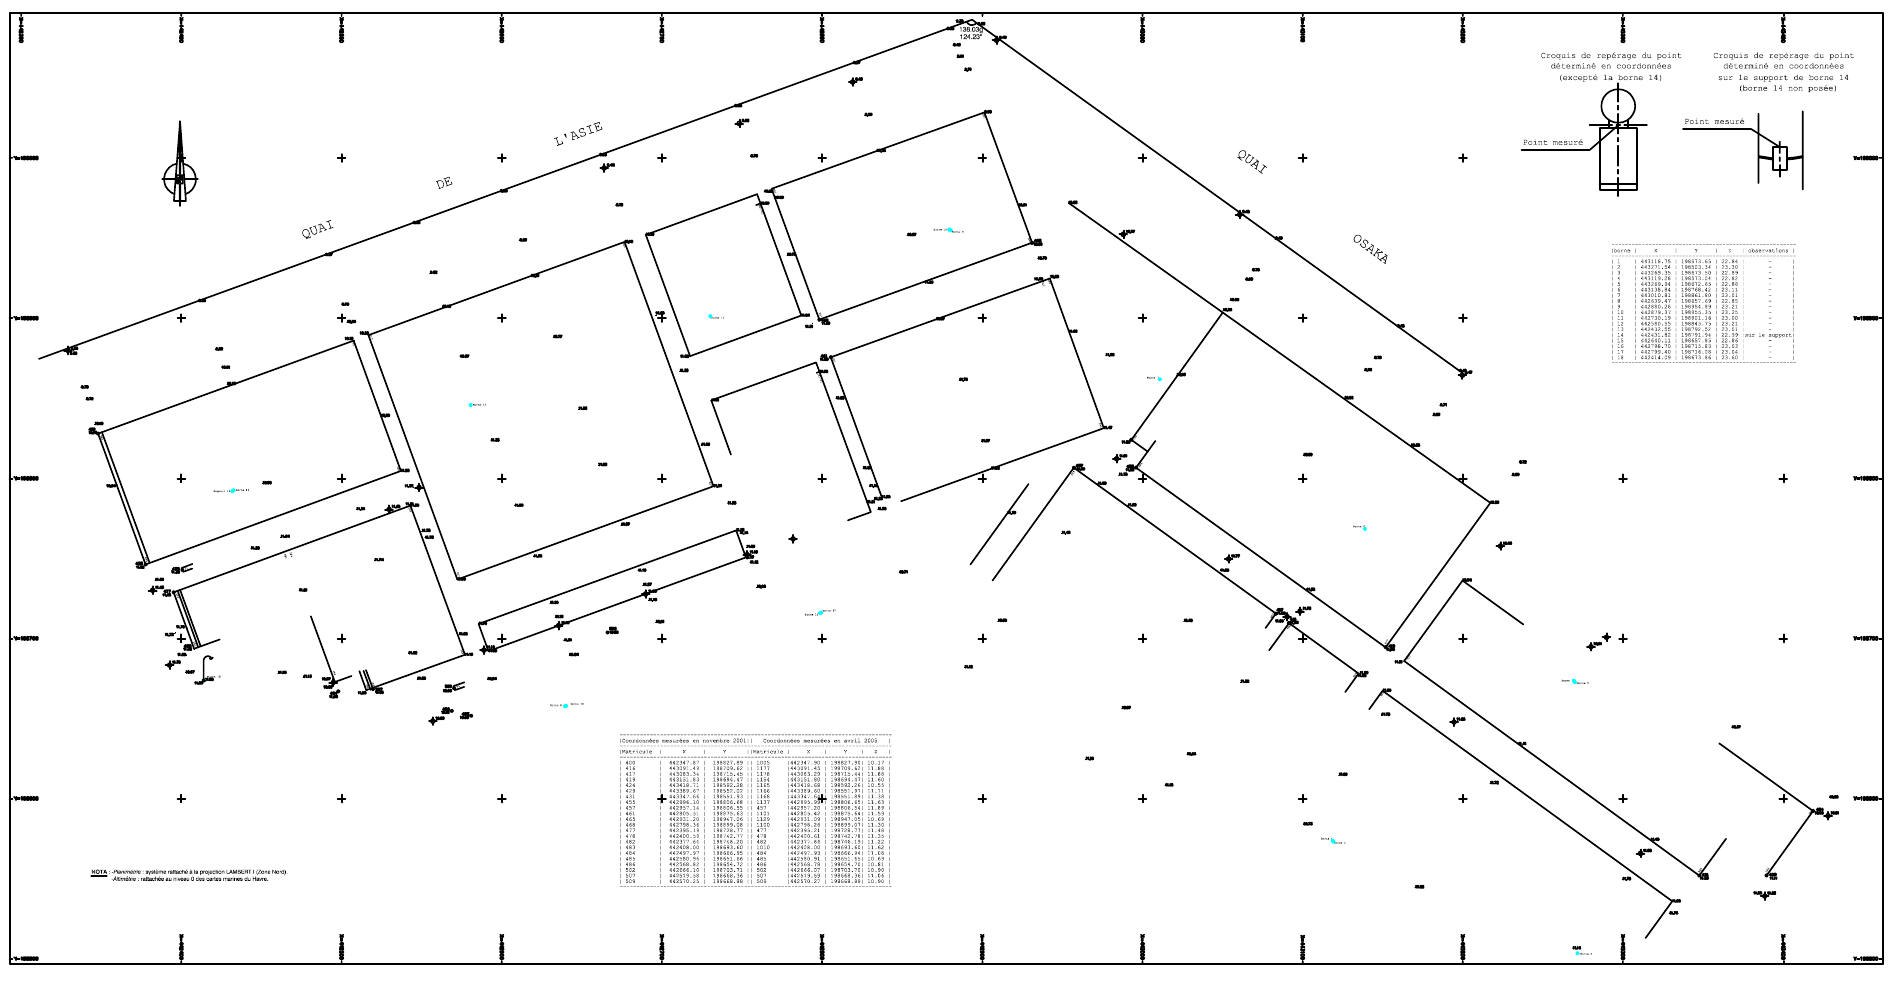
\includegraphics[height=.50\textheight]{fig/planNormandieZ.png}
    \end{center}
      \pause
      \item Straddle carriers models characteristics
      \pause
      \item Laser system data
    \end{itemize}

    
\end{frame}
\begin{frame}{Retrieving data (2)}
    \begin{center}
      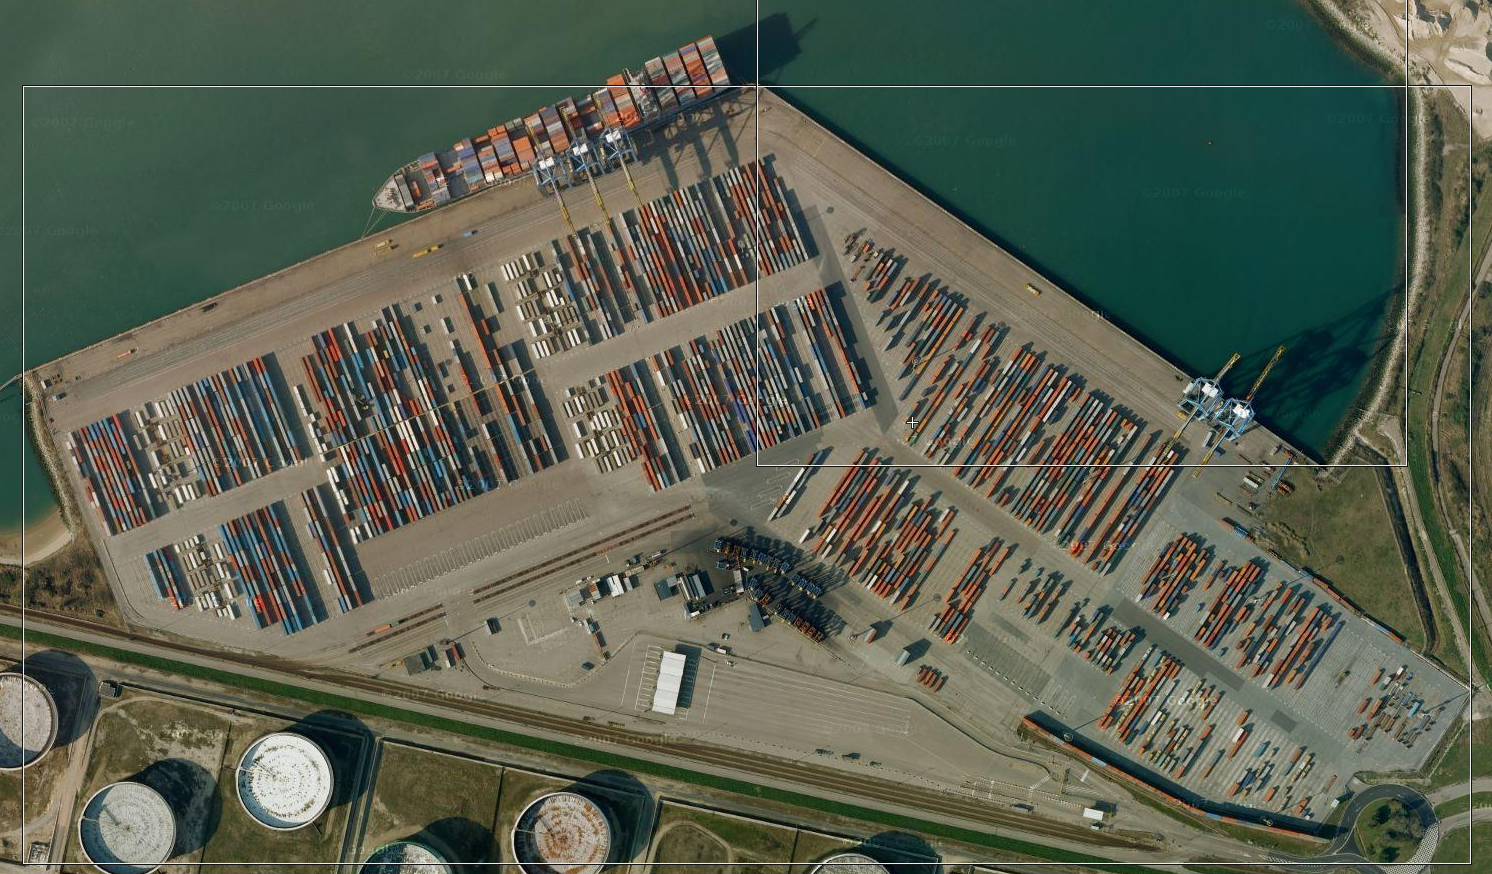
\includegraphics[height=.70\textheight]{fig/NormandieZ.png} \\
      \tiny \textit{Terminal de Normandie}, Le Havre, France (wikimapia.org)
    \end{center}
\end{frame}
\begin{frame}{Retrieving data (3)}
   \begin{center}
      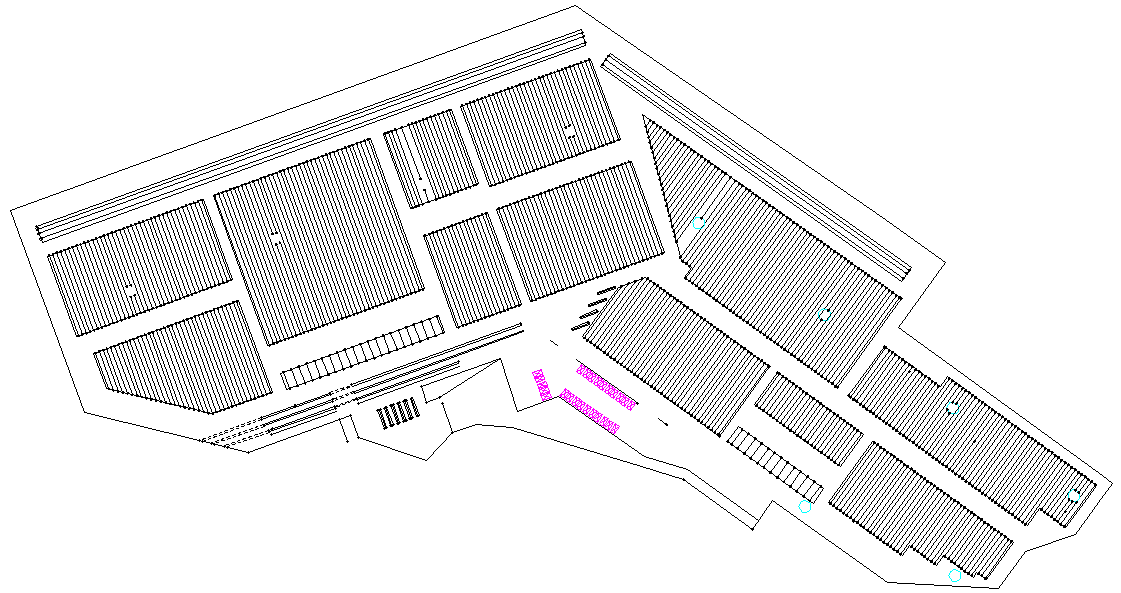
\includegraphics[height=.70\textheight]{fig/planTerminalDetailleBlanc.png} \\
       \tiny Detailed plan of the \textit{Terminal de Normandie}, Le Havre, France
    \end{center}
\end{frame} 

\begin{frame}{Data Structuration}
  \begin{block}{XML formalization}
    \begin{itemize}
      \item Simplicity
      \item Clarity of the data
      \item Personalization
      \item Easy navigation
    \end{itemize}
   \end{block}
   
  \begin{center}   
    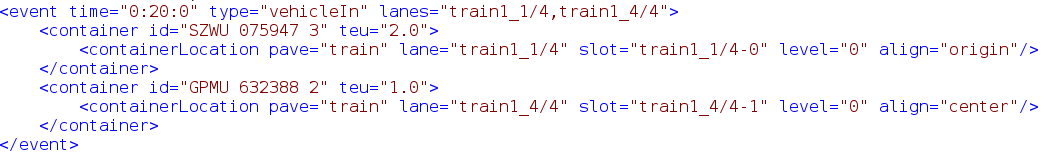
\includegraphics[width=.90\textwidth]{fig/structureXML.png}
   \end{center}
\end{frame}


\section{Simulated optimization problems}
\subsection*{Terminal architecture}
\begin{frame}{Terminal Configuration}
  \begin{block}{Objective :}
    Testing the structure of a terminal
  \end{block}
  \pause
  Measuring the impact of the terminal architecture on: 
  \begin{itemize}
  \pause
   \item the exploitation costs
  \pause
   \item the quality of service
  \end{itemize}
 \end{frame}
\subsection*{Dangerous containers positioning}
\begin{frame}{Dangerous containers positioning}
  \begin{block}{Objective:}
    Finding a matching location for a container
  \end{block}
  \pause
  The problem consists in choosing a location reducing the handling distances and complying with the safety standards
  \end{frame}

    \subsection*{Missions scheduling}
\begin{frame}{Dynamic scheduling}
 \begin{itemize}   
   \item For a straddle carrier, a mission consists in moving a container
   \pause
    \item 2 phases : pickup and delivery
    \pause
    \item 2 time windows
    \pause
      \begin{itemize}
	\item At least 1 soft, 2 at the most
	\pause
	\item Generally 1 hard
      \end{itemize} 
    \pause
    \item $m$ straddle carriers
    \item $n$ missions
\end{itemize}
\pause
\begin{block}{ Modeled problem: }
   	\begin{minipage}[]{\columnwidth}
		Dynamic version of a missions scheduling and allocating problem %Version dynamique d'un problème d'ordonnancement et d'affectation de missions
	\end{minipage}
  \end{block}
  \end{frame}

\subsection*{Vehicles routing}
\begin{frame}{Routing problem}
    \begin{block}{Original problem: }
      To minimize the travel distance of the straddle carriers to reduce the exploitation costs
    \end{block}
\pause
    \begin{block}{Routing problem on a container terminal:}
       \begin{itemize} 
	  \item Roads : non FIFO arcs
	  \item Lanes : FIFO arcs with unit capacity
	  \item The speed of a straddle carrier depends on its location
	
	\end{itemize}
	\pause
	\begin{center}
	    $\Rightarrow$ To minimize the travel time to reduce the costs and to maintain a sufficient quality of service
	  \end{center}
    \end{block}
  \end{frame}

\section{Conclusion}
    \begin{frame}{Conclusion \& Outlook}
    \begin{itemize}
     \item Validation process
    \pause
     \item In collaboration with EADS/Astrium to integrate a 3D visualization add-on
    \pause
     \item Looking for partners to: 
	\begin{itemize}
	 \item collect data (container terminal architectures, data sets)
	 \item test optimization algorithms (missions scheduling, vehicle routing)
	\end{itemize}
    \end{itemize}
  \pause
  \begin{center}
  contact : gaetan.lesauvage@litislab.eu
  \end{center}
  \end{frame}

\end{document}
